% ============================ Enrico Ribiani 16-03-2021 ====================================================================
% Base per i documenti  
\documentclass[12pt]{article}
% ------------ pacchetti necessari ----------------
\usepackage[a4paper, total={6in, 8in},margin=1in]{geometry} % formattazione decente della pagina
\usepackage{graphicx}                            % need for figure
\usepackage{amsmath}
\usepackage{amsfonts}                            % if you want the fonts
\usepackage{amssymb}                             % if you want extra symbols
\usepackage{graphicx}  
\renewcommand{\figurename}{Figura}  
\renewcommand{\contentsname}{Indice}                        % need for figures
\usepackage{mathptmx}
\usepackage{float}                               % serve per mettere tabelle e immagini dove si vuole 
\usepackage[utf8]{inputenc}
\usepackage{textcomp}
\usepackage[hang,flushmargin,bottom]{footmisc}   % footnote format
\usepackage{fancyhdr, lastpage}
\usepackage{titlesec}
\usepackage[table,dvipsnames]{xcolor}
%\pagestyle{fancy}
%\renewcommand{\headrulewidth}{0pt}
%\renewcommand*\contentsname{Indice}
\titleformat{\section}{\normalsize\bfseries}{\thesection.}{1em}{}	% required for heading numbering style
\titleformat*{\section}{\Large\bfseries}
\titleformat*{\subsection}{\large\bfseries}
%\usepackage{siunitx}
%\usepackage{tikz}
\usepackage{circuitikz}
\usepackage{multicol}
%\usepackage[siunitx]{circuitikz}
\usepackage{multirow}
\usepackage{tikz}
\usepackage{amsmath}
\usetikzlibrary{angles,quotes}
\usepackage{placeins}

\usepackage{wasysym}
%===================links=================
\usepackage{hyperref}
\hypersetup{
    colorlinks=true,
    linkcolor=darkgray,
    filecolor=Green,      
    urlcolor=Cyan,
    pdftitle={relazione-elt},
    pdfpagemode=FullScreen,
    }
%===================inizio pagina del titolo=================
\begin{document}
    \begin{titlepage}
    \begin{center}
% ------------------ inizio immagine logo ----------
\begin{figure}
    \centering
   % 
\includegraphics[scale=1.5]{~/Documenti/latec/logo.png}
    \label{fig:logo}
\end{figure}
% ------------------ fine immagine logo ----------
% ------------------ fine immagine logo ----------
-------------------------------------------------------------------------------------\\
\vspace{2\baselineskip}
\large Prova n°4
\hfill
\large $5^a$   AUB\\
\begin{flushleft}
    \large Enrico Ribiani\\
    \large Giuliano Holler\\
    %\large Gruppo 11\\
\end{flushleft}


\vfill

\Huge{\textbf{Tiristori scr e triac}}\\
\vfill
\vfill
\large{26-01-2023}
\end{center}
%=============== fine pagina titolo ===============
\end{titlepage}
\tableofcontents
\newpage
\vskip 1cm
\section{Scopo}
Lo scopo di questa esperienza laboratoriale è di osservare il comportamento di un scr e di un triac in diverse condizioni.
\noindent
\section{Tiristori SCR}
    \subsection{Schema scr} \label{Schema scr}
\begin{flushleft}
    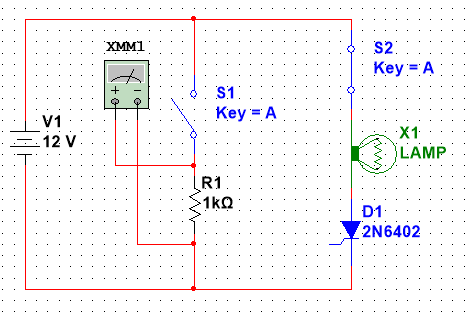
\includegraphics[scale=0.8]{schema-scr-A}
    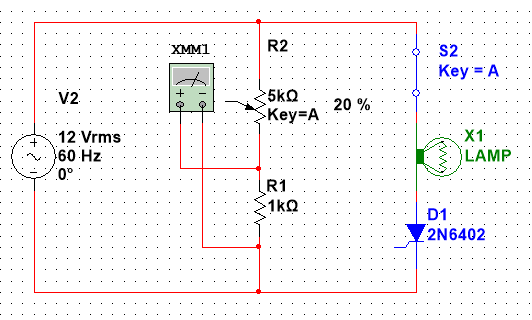
\includegraphics[scale=0.8]{schema-scr-B}
\end{flushleft}
    \subsection{Materiale e Strumenti}
    \begin{multicols}{2}
    \begin{itemize}
    \item Fili di collegamento
    \item Breadboard
    \item Resistenza da $1k\Omega$
    \item Potenziometro da $5k\Omega$
    \item SCR \textit{}
    \item Lampadina
    \end{itemize}
    \vfill\null
    \columnbreak
    \begin{itemize}
    \item Multimetro
    \item Generatore AC
    \item Alimentazione DC 
    \end{itemize}
    \vfill\null
    \end{multicols}
    \subsection{Contenuti teorici}
    Il raddrizzatore controllato a silicio (\textit{SCR} la sigla inglese) o tiristore è un componente a tre morsetti, uno di controllo detto \textit{gate} e due di potenza chiamati \textit{A}(+) e \textit{K}(-).\\
    Questo componente ha una funzione ON-OFF  controllata dalla tensione sul gate ($V_G$) che causerà la corrente $I_G$.\\
    Una volta innescato il tiristore rimarrà in conduzione fino a quando la corrente che attraversa il componente è maggiore di $I_L$ stabilita dal costruttore, anche in assenza di $I_G$.\\
Per far tornare il tiristore nella fase di interdizione è necessario o ridurre la corrente che va da un morsetto di potenza all'altro o polarizzare inversamente \textir{G} con una tensione \textit{$V_G$} negativa. \\   \noindent

        \subsubsection{Descrizione della prova}
        La prova verrà realizzata andando a osservare il comportamento del tiristore in due circuiti diversi riportati nella sezione \ref{Schema scr} andando a misurare in entrambi la tensione e corrente sul componente.\\
        Il primo circuito verrà testato sia in corrente alternata che in corrente continua.\\
        \subsubsection{Raccolta dei dati}
        \begin{table}[ht]
        \centering
          \begin{tabular}{|c|c|} 
        \hline
        \rowcolor{RoyalBlue} $V_{ak}$ & $I_{ak}$& 
        \hline
        \rowcolor{CornflowerBlue} $11,22V$ & $11,36mA$ &
        \hline
    \end{tabular}
            \caption{Circuito 1 DC}
            \label{tab:Circuito 1 DC}
        \end{table}
        \\
                \begin{table}[ht]
        \centering
          \begin{tabular}{|c|c|} 
        \hline
        \rowcolor{ForestGreen} $V_{ak}$ & $I_{ak}$& 
        \hline
        \rowcolor{LimeGreen} $10,3V$ & $10,4mA$ &
        \hline
    \end{tabular}
            \caption{Circuito 1 AC}
            \label{tab:Circuito 1 AC}
        \end{table}
         \\
                \begin{table}[ht]
        \centering
          \begin{tabular}{|c|c|} 
        \hline
        \rowcolor{Dandelion} $V_{ak}$ & $I_{ak}$& 
        \hline
        \rowcolor{Goldenrod} $2,38V$ & $1,5mA$ &
        \hline
    \end{tabular}
            \caption{Circuito 2 AC}
            \label{tab:Circuito 2 AC}
        \end{table}

        \subsubsection{Commento dei dati raccolti}
        Dai dati raccolti nelle tabelle possiamo notare che i valori ricavati dal primo circuito sono molto simili anche se alimentati da tensioni diverse ma con lo stesso valore efficace.\\
        I dati ricavati dal secondo circuito invece risultano di molto inferiori a causa del cambiamento effettuato nel circuito con l'aggiunta del potenziometro.\\ %\textcolor{Red}{\textbf{NON SO PERCHÈ}}.\\
        Inoltre la missura è stata effettuata con il minimo valore di tensione che riesce ad accendere la lampadina.\\
        \newline
        NB:Il prrimo circuito quando alimentato da corrente alternata accende la lampadina solamente con  il pulsante chiuso altrimenti il tiristore si polarizzerebbe negativamente all'istante.\\
        \subsubsection{Calcoli}
        Per calcolare R abbiamo utilizzato il valore di alimentazione che in questo caso è anche $V_G$ e il valore desiderato di $I_G$.\\
        $R=\frac{V_G}{I_G}$
    \subsection{Analisi critica dei risultati e conclusioni}
    Osservando il comportamento del circuito e analizzando i risultati ottenuti possiamo dire che il circuito si è comportato esattamente come ci si aspettava segueno la teoria di funzionamento del componente.\\
%-----------------------------------------
\section{Triac}
\subsection{Schema triac}
    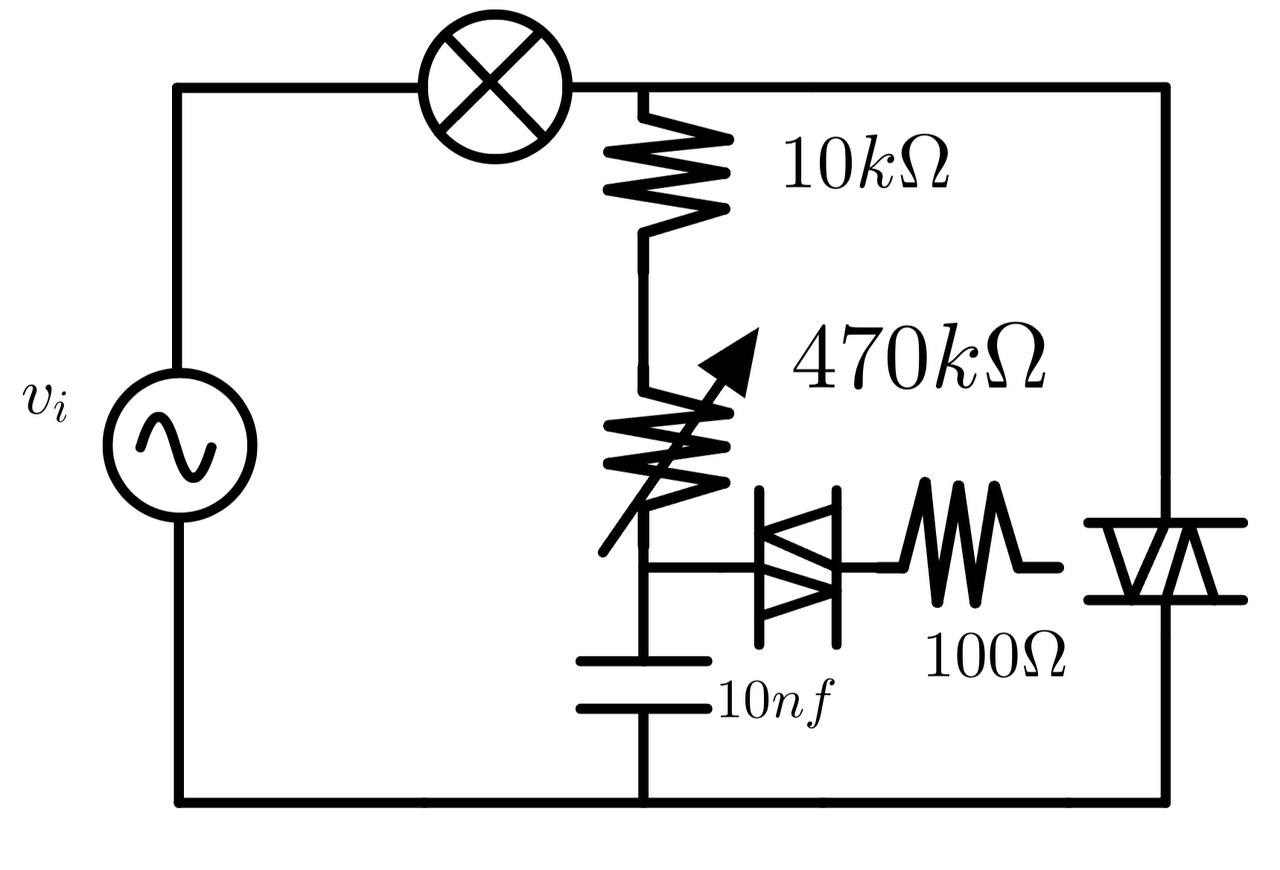
\includegraphics[scale=0.2]{schema-triac}
    \subsection{Materiale e Strumenti}
    \begin{multicols}{2}
    \begin{itemize}
    \item Fili di collegamento
    \item Breadboard
    \item Resistenza da $10k\Omega$
    \item Resistenza da $100k\Omega$
    \item Potenziometro da $470k\Omega$
    \item Triac \textit{TIC216M}
    \item Diac
    \item Condensatore $100nF$
    \item Lampadina
    \end{itemize}
    \vfill\null
    \columnbreak
    \begin{itemize}
    \item Multimetro
    \item Generatore AC
    \item Alimentazione DC 
    \end{itemize}
    \vfill\null
    \end{multicols}
    \subsection{Contenuti teorici}
    Il \textbf{Triac} è un componente elettronico, di tipo semiconduttore, specificamente progettato per controllare carichi in corrente alternata, si tratta di un dispositivo a tre terminali, di cui due sono detti anodi e sono la via di passaggio per la corrente controllata, mentre il terzo, definito gate, è l'ingresso di controllo.\\
    Idealmente il Triac equivale a due SCR collegati in antiparallelo con il gate in comune.\\
    Ciascun elemento conduce solamente nel semiperiodo dell'onda in cui è polarizzato direttamente, da quando viene applicato un impulso di corrente al gate fino al passaggio per lo zero della corrente.\\
        \subsubsection{Descrizione della prova}
        La prova consiste nel vedere la variazione della luminosità della lampada nel circuito, la quale rappresenterà la variazione dell’angolo di innesto del Triac data dalla variazione del trimmer.\\
Viene applicata una corrente tale da fare in modo che il triac conduca, questa corrente verrà poi mantenuta dal condensatore, inoltre si verificherà la variazione di tensione nelle semionde tramite un oscilloscopio.\\
\\
    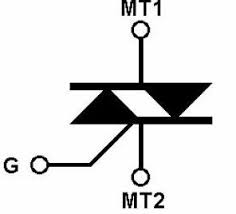
\includegraphics[scale=0.4]{triac}

        \subsubsection{Raccolta dei dati}
        \begin{figure}[|h]
            \centering
            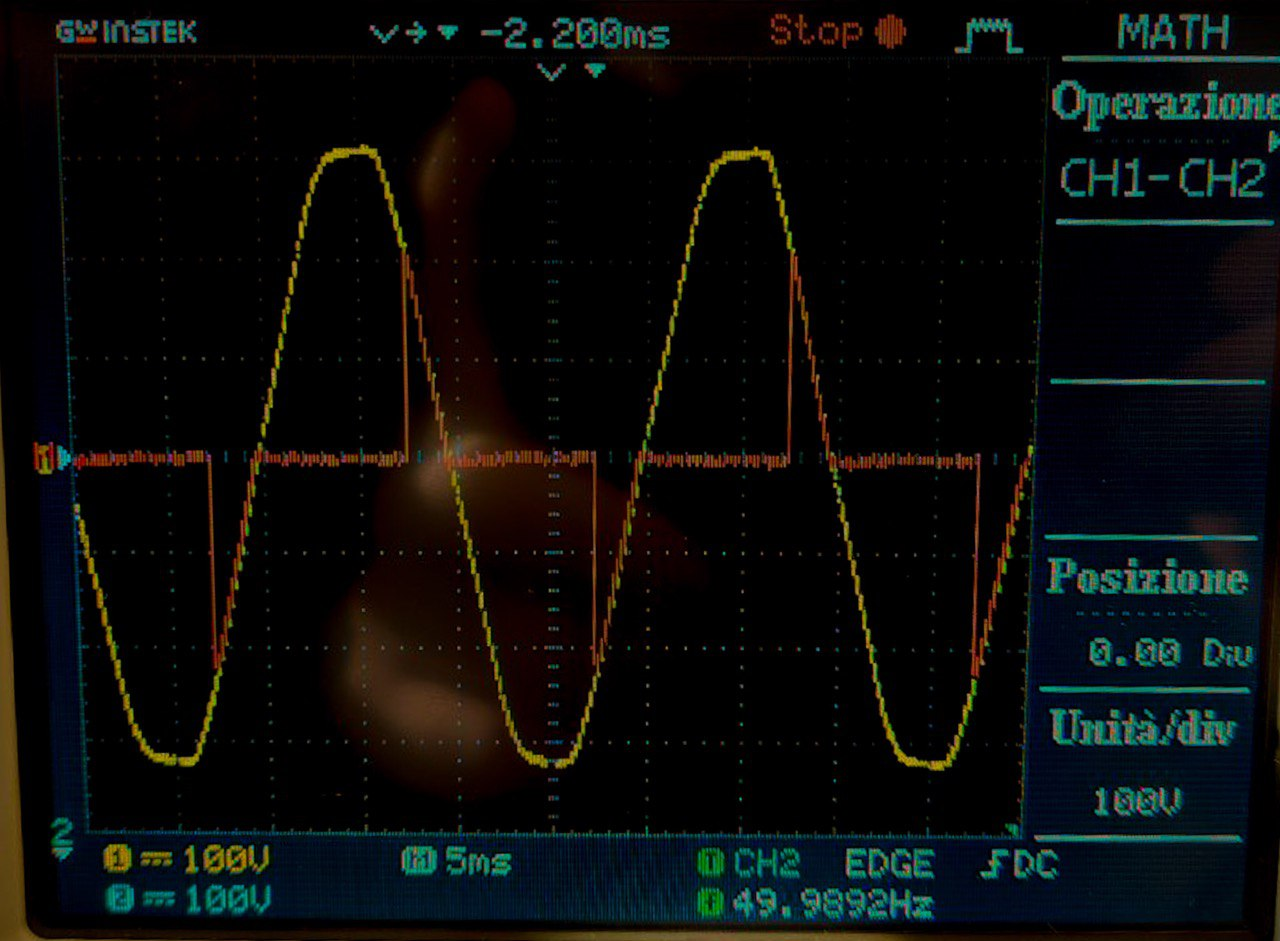
\includegraphics[scale=0.12]{oscilloscopio.jpg}
            \caption{Oscilloscopio}
            \label{fig:Oscilloscopio}
        \end{figure}
        \subsubsection{Commento dei dati raccolti}
        Da queste immagini si può capire in modo chiaro il diverso funzionamento del Triac in base alla variazione della corrente ad esso applicata.\\ Si riesce a vedere bene il punto di innesto anche se poco preciso dato dalla scala elevata dello oscilloscopio e dal rumore della tensione di rete.\\

        \subsubsection{Calcoli}
        $V_L=V_{ch1}-V_{ch2}\\$
    \subsection{Analisi critica dei risultati e conclusioni}
    Osservando il comportamento del circuito e analizzando i risultati ottenuti possiamo dire che il circuito si è comportato esattamente come ci si aspettava segueno la teoria di funzionamento del componente.\\
\end{document}
\end{document}